\pagebreak
\section{Truncation Error Analysis}
Use the method of undetermined coefficients to derive a finite-difference approximation to the second derivative of $u$ at point 0, $u_{xx}|_0$, using $u$ values at points 0,1,2 on a uniform grid.  Repeat this with the addition of $u$ at point 3.  In both cases, determine the order of accuracy of your formula.

    \begin{figure}[h]
        \centering
        

\tikzset{every picture/.style={line width=0.75pt}} %set default line width to 0.75pt        

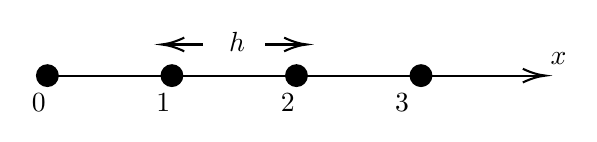
\begin{tikzpicture}[x=0.75pt,y=0.75pt,yscale=-1,xscale=1]
%uncomment if require: \path (0,300); %set diagram left start at 0, and has height of 300

%Straight Lines [id:da22033664838285616] 
\draw    (165,75) -- (403,75) ;
\draw [shift={(405,75)}, rotate = 180] [color={rgb, 255:red, 0; green, 0; blue, 0 }  ][line width=0.75]    (10.93,-3.29) .. controls (6.95,-1.4) and (3.31,-0.3) .. (0,0) .. controls (3.31,0.3) and (6.95,1.4) .. (10.93,3.29)   ;
%Shape: Circle [id:dp9884543751049439] 
\draw  [fill={rgb, 255:red, 0; green, 0; blue, 0 }  ,fill opacity=1 ] (160,75) .. controls (160,72.24) and (162.24,70) .. (165,70) .. controls (167.76,70) and (170,72.24) .. (170,75) .. controls (170,77.76) and (167.76,80) .. (165,80) .. controls (162.24,80) and (160,77.76) .. (160,75) -- cycle ;
%Shape: Circle [id:dp2915366064031737] 
\draw  [fill={rgb, 255:red, 0; green, 0; blue, 0 }  ,fill opacity=1 ] (220,75) .. controls (220,72.24) and (222.24,70) .. (225,70) .. controls (227.76,70) and (230,72.24) .. (230,75) .. controls (230,77.76) and (227.76,80) .. (225,80) .. controls (222.24,80) and (220,77.76) .. (220,75) -- cycle ;
%Shape: Circle [id:dp739979693411948] 
\draw  [fill={rgb, 255:red, 0; green, 0; blue, 0 }  ,fill opacity=1 ] (340,75) .. controls (340,72.24) and (342.24,70) .. (345,70) .. controls (347.76,70) and (350,72.24) .. (350,75) .. controls (350,77.76) and (347.76,80) .. (345,80) .. controls (342.24,80) and (340,77.76) .. (340,75) -- cycle ;
%Shape: Circle [id:dp09438495424307014] 
\draw  [fill={rgb, 255:red, 0; green, 0; blue, 0 }  ,fill opacity=1 ] (280,75) .. controls (280,72.24) and (282.24,70) .. (285,70) .. controls (287.76,70) and (290,72.24) .. (290,75) .. controls (290,77.76) and (287.76,80) .. (285,80) .. controls (282.24,80) and (280,77.76) .. (280,75) -- cycle ;
%Straight Lines [id:da9634228986430384] 
\draw    (270,60) -- (288,60) ;
\draw [shift={(290,60)}, rotate = 180] [color={rgb, 255:red, 0; green, 0; blue, 0 }  ][line width=0.75]    (10.93,-3.29) .. controls (6.95,-1.4) and (3.31,-0.3) .. (0,0) .. controls (3.31,0.3) and (6.95,1.4) .. (10.93,3.29)   ;
%Straight Lines [id:da5444183929083122] 
\draw    (222,60) -- (240,60) ;
\draw [shift={(220,60)}, rotate = 0] [color={rgb, 255:red, 0; green, 0; blue, 0 }  ][line width=0.75]    (10.93,-3.29) .. controls (6.95,-1.4) and (3.31,-0.3) .. (0,0) .. controls (3.31,0.3) and (6.95,1.4) .. (10.93,3.29)   ;

% Text Node
\draw (406,62.4) node [anchor=north west][inner sep=0.75pt]    {$x$};
% Text Node
\draw (251,52.4) node [anchor=north west][inner sep=0.75pt]    {$h$};
% Text Node
\draw (156,82.4) node [anchor=north west][inner sep=0.75pt]    {$0$};
% Text Node
\draw (216,82.4) node [anchor=north west][inner sep=0.75pt]    {$1$};
% Text Node
\draw (276,82.4) node [anchor=north west][inner sep=0.75pt]    {$2$};
% Text Node
\draw (331,82.4) node [anchor=north west][inner sep=0.75pt]    {$3$};


\end{tikzpicture}

        \caption{Undetermined coefficients on a uniform grid.}
    \end{figure}

\vspace{-0.2in}
\begin{align*}
    \shortintertext{Firstly start with the equation for the method of undetermined coefficients,}
    \frac{d^2u}{dx^2} = \sum_{j=0}^{2} & = a_2u_2 + a_1u_1 + a_0u_0\\
    \shortintertext{Conducting Taylor-Expansions for $u_2,\ u_1,\ u_0$ gives,}
        & = a_2 \underbrace{\left(u_0 + (2h)\frac{du}{dx} + \frac{1}{2}(2h)^2\frac{d^2u}{dx^2} + \frac{1}{6}(2h)^3\frac{d^3}{dx^3} + \ldots \right)}_{\text{Taylor-Expansion about $u_2$}}\\
        & + a_1\underbrace{\left(u_0 + h\frac{du}{dx} + \frac{1}{2}h^2\frac{d^2u}{dx^2} + \frac{1}{6}h^3\frac{d^3u}{dx^3} + \ldots \right)}_{\text{Taylor-Expansion about $u_1$}}\\
        & + a_0u_0\\
    \shortintertext{Grouping all the terms gives,}
        & = \left(a_2 + a_1 + a_0\right)u_0 + \left(2a_2 + a_1\right)h\frac{du}{dx}\\
        & + \left(2a_2 + \frac{1}{2}a_1\right)h^2\frac{d^2u}{dx^2} + \left(\frac{4}{3}a_2 + \frac{1}{6}a_1\right)h^3\frac{d^3u}{dx^3} + \ldots \mathcal{O}(h^4)\\
    \shortintertext{With three unknowns and three equations to solve for $a_0,\ a_1,\ a_2$ writing out in matrix form is,}
     & \begin{bmatrix}
        0\\
        0\\
        \frac{1}{h^2}
    \end{bmatrix} = \begin{bmatrix}
        a_2 + a_1 + a_0\\
        2a_1 + a_1\\
        2a_2 + \frac{1}{2}a_1
    \end{bmatrix}\\
    \shortintertext{Solving for $a_0,\ a_1,\ a_2$ then becomes,}
\end{align*}

\vspace{-0.5in}
\begin{equation*}
    \boxed{a_0 = \input{q2/p1_a0},\quad  a_1 = \input{q2/p1_a1},\quad  a_2 = \input{q2/p1_a2}}
\end{equation*}

\vspace{-0.35in}
\begin{align*}
    \shortintertext{Expanding the expression further gives that to the next higher term $\frac{d^3}{dx^3}$ gives,}
    0 + \frac{1}{6}a_1 + \frac{4}{3}a_2 & = h^3\frac{d^3}{dx^3}\\
    \shortintertext{Substituting in the $a$ values from above,}
    -\frac{1}{3h^3} + \frac{4}{3h^2} & = h^3\frac{d^3}{dx^3},\quad 1 = h\frac{d^3u}{dx^3}\\
    \frac{d^2u}{dx^2} & = \frac{u_2 -2u_1 + u_0}{h^2} + h\frac{d^3u}{dx^3}\\
\end{align*}

\vspace{-0.25in}
\begin{fminipage}{0.8\linewidth}
    \centering
    \textbf{Shown above this is first-order accurate since the error is $\bf \mathcal{O}(h)$.}
\end{fminipage}

\pagebreak
\begin{align*}
    \shortintertext{Repeating with the addition of $u$ at point 3 gives,}
    \frac{d^2u}{dx^2} = \sum_{j=0}^{3} & = a_3u_3 + a_2u_2 + a_1u_1 + a_0u_0\\
    \shortintertext{Conducting Taylor-Expansions for $u_3,\ u_2,\ u_1,\ u_0$ gives,}
    & = a_3 \underbrace{\left(u_0 + (3h)\frac{du}{dx} + \frac{1}{2}(3h)^2\frac{d^2u}{dx^2} + \frac{1}{6}(3h)^3\frac{d^3u}{dx^2} + \ldots\right)}_{\text{Taylor-Expansion about $u_3$}}\\
    & + a_2 \underbrace{\left(u_0 + (2h)\frac{du}{dx} + \frac{1}{2}(2h)^2\frac{d^2u}{dx^2} + \frac{1}{6}(2h)^3\frac{d^3}{dx^3} + \ldots \right)}_{\text{Taylor-Expansion about $u_2$}}\\
    & + a_1\underbrace{\left(u_0 + h\frac{du}{dx} + \frac{1}{2}h^2\frac{d^2u}{dx^2} + \frac{1}{6}h^3\frac{d^3u}{dx^3} + \ldots \right)}_{\text{Taylor-Expansion about $u_1$}}\\
    & + a_0u_0\\
    \shortintertext{Grouping all the terms gives,}
    & = \left(a_3 + a_2 + a_1 + a_0\right)u_0 + \left(3a_3 + 2a_2 + a_1\right)h\frac{du}{dx} \\
    & + \left( \frac{9}{2}a_3 + 2a_2 + \frac{1}{2}a_1  \right)h^2\frac{d^2u}{dx^2} + \left( \frac{9}{2}a_3 + \frac{4}{3}a_2 + \frac{1}{6}a_1 \right)h^3\frac{d^3u}{dx^3}\\
    & + \ldots \mathcal{O}(h^5)\\
    \shortintertext{With four unknowns and four equations to solve for $a_0,\ a_1,\ a_2,\ a_3$ writing out in matrix form is,}
    & \begin{bmatrix} 0\\ 0\\ \frac{1}{h^2}\\ 0\\\end{bmatrix} = \begin{bmatrix}
        a_3 + a_2 + a_1 + a_0\\
        3a_3 + 2a_2 + a_1\\
        \frac{9}{2}a_3 + 2a_2 + \frac{1}{2}a_1\\
        \frac{9}{2}a_3 + \frac{4}{3}a_2 + \frac{1}{6}a_1
    \end{bmatrix}
    \shortintertext{Solving for $a_0,\ a_1,\ a_2,\ a_3$ then becomes,}
\end{align*}

\vspace{-0.5in}
\begin{equation*}
    \boxed{a_0 = \input{q2/p2_a0},\quad  a_1 = \input{q2/p2_a1},\quad  a_2 = \input{q2/p2_a2},\quad a_3 = \input{q2/p2_a3}}
\end{equation*}

\vspace{-0.3in}
\begin{align*}
    \shortintertext{Expanding the expression further gives that to the next higher term $\frac{d^3}{dx^3}$ gives,}
    0 + \frac{1}{24}a_1 + \frac{16}{24}a_2 + \frac{81}{24}a_3 & = -\frac{11}{12h^2}\left(h^4\frac{d^4}{dx^4}\right)\\
    \shortintertext{Substituting in the $a$ values from above,}
    \frac{d^2u}{dx^2} & = \frac{2u_0 - 5u_1 + 4u_2 - u_3}{h^2} + h^2\frac{d^4u}{dx^4}\\
\end{align*}

\vspace{-0.25in}

\begin{fminipage}{0.8\linewidth}
    \centering
    \textbf{Shown above this is second-order accurate since the error is $\bf \mathcal{O}(h^2)$.}
\end{fminipage}